\chapter{Aktuální řešení}

V této kapitole stručně popíši verzi aplikace, která byla vytvořena v rámci bakalářské práce \cite{bp} a kterou budu v praktické části rozšiřovat. Popíši implementované funkční i nefunkční požadavky, použité technologie a také konfiguraci prostředí a způsob nasazování. Na závěr stručně shrnu, jaké možné plány na rozšíření byly v rámci bakalářské práce nastíněny.

\section{Implementované požadavky}

\subsection{Implementované funkční požadavky}

V této podsekci shrnu implementované funkční požadavky. Součástí této podsekce je také původní logický datový model aplikace z bakalářské práce \cite{bp} na obrázku~\ref{fig:db-model} pro lepší pochopení domény.

Shrnutí funkčních požadavků \cite{bp}:
\begin{itemize}
    \item \textbf{evidence klientů:} evidování základních informací o klientovi,
    \item \textbf{evidence lekcí klientů:} evidování základních informací o lekcích (včetně stavů účasti všech účastníků a stavu jejich platby za danou lekci), lekce mohou být pro jednotlivce nebo pro skupiny, každá náleží nějakému kurzu,
    \item \textbf{evidence předplacených lekcí:} předplacená lekce je řešená jako lekce, která nemá datum a čas konání,
    \item \textbf{evidence kurzů a stavů účasti:} pro použití při evidenci lekcí,
    \item \textbf{přehled lekcí pro aktuální den:} zobrazení pro dnešní lekce (kromě zrušených),
    \item \textbf{karta klienta a skupiny}: zobrazení všech informací o klientovi/skupině včetně všech lekcí,
    \item \textbf{upozornění na platbu příště:} když už klient nemá žádné předplacené lekce, zobrazí se u poslední placené lekce upozornění na fakt, že má příště zaplatit,
    \item \textbf{pořadové číslo lekce:} u lekce se zobrazí (automaticky vypočítáno), o kolikátou navštívenou lekci v pořadí se jedná,
    \item \textbf{týdenní přehled:} zobrazení lekcí jako v diáři.
\end{itemize}

\begin{figure}[h]\centering
	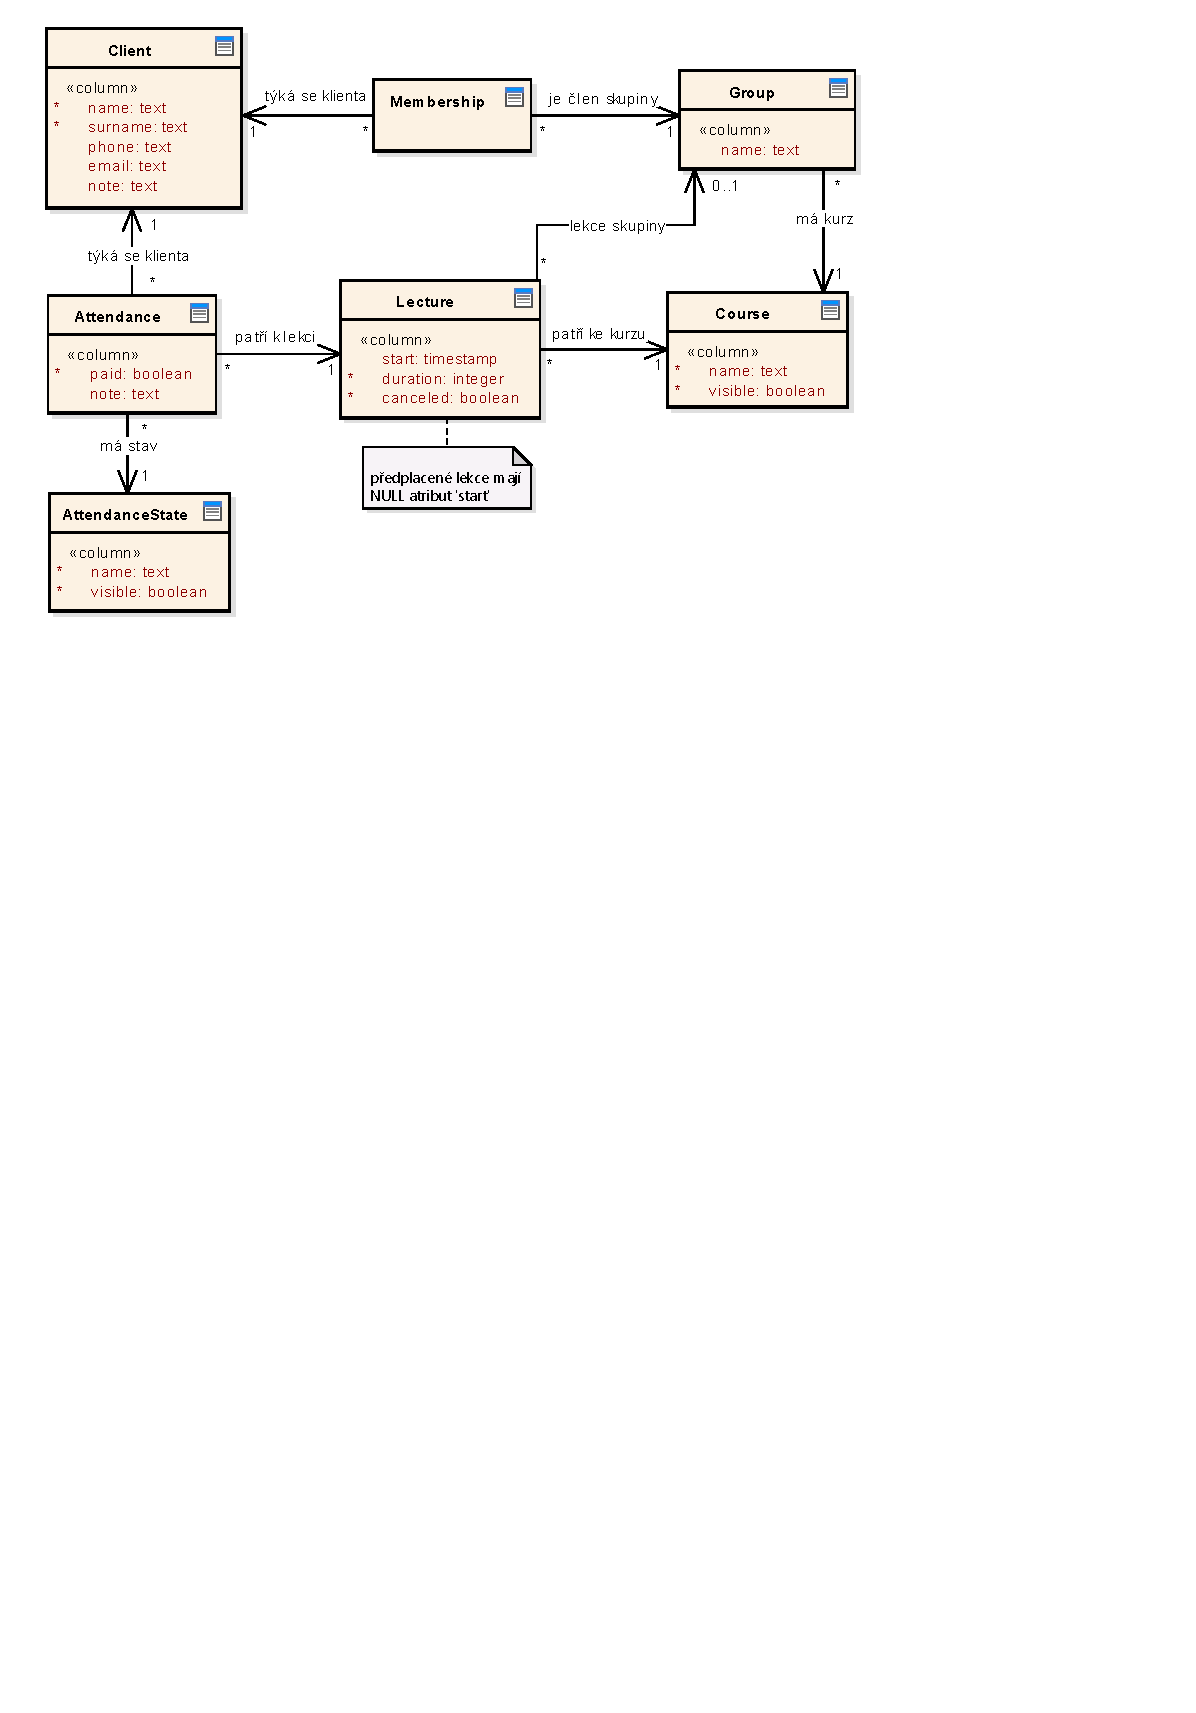
\includegraphics[width=1\textwidth]{img/bp/db-model}
	\caption[Logický datový model z bakalářské práce]{Logický datový model z bakalářské práce \cite{bp}}\label{fig:db-model}
\end{figure}

\subsection{Implementované nefunkční požadavky}

Následuje shrnutí nefunkčních požadavků \cite{bp}:
\begin{itemize}
    \item \textbf{kompatibilita s webovými prohlížeči:} aplikace je plně funkční a kompatibilní s běžnými webovými prohlížeči (Google Chrome, Mozilla Firefox, Microsoft Edge, Apple Safari) v posledních verzích, důraz je především kladen na desktopový prohlížeč Mozilla Firefox, na kterém se aplikace používá primárně,
    \item \textbf{podpora široké škály zařízeních:} aplikace je responzivní a korektně se zobrazuje na všech zařízeních používaných lektorkou -- iPad s iOS~13.3 a 9,7palcovým displejem, Nokia~5 s Androidem~9.0 a 5,2palcovým~displejem, notebook s Windows~10 s rozlišením 1920~×~1080 a 15,6palcovým~displejem,
    \item \textbf{připravenost na rozšíření a údržbu}: kód byl tvořen s důrazem na budoucí možná rozšíření (např. použití konstant, respektování principu DRY (\enquote{Don\textquotesingle t repeat yourself}) ad.),
    \item \textbf{bezpečnost:} JWT (JSON Web Token) autentizace a další produkční konfigurace pro zabezpečení aplikace,
    \item \textbf{srozumitelné a jednoduché rozhraní aplikace:} iterativní návrh a implementace UI za neustálé spolupráce s lektorkou pro dosažení co nejlepší použitelnosti.
\end{itemize}


\section{Použité technologie}

\subsection{Serverová část}

Serverová část aplikace \cite{bp} je napsána v Pythonu~3.6.5 s webovým frameworkem \href{https://www.djangoproject.com/}{Django~2.0.5}. Pro správu závislostí se používá pouze jednoduchý soubor \verb|requirements.txt| obsahující specifikace přesných verzí knihoven (bez povolení jakkoliv malých aktualizací). 

Aplikace vystavuje REST~API postavené na frameworku \href{https://www.django-rest-framework.org/}{Django~REST~framework~3.8.2}. Na produkci se používá webový server \href{http://gunicorn.org/}{Gunicorn~19.8.1} spolu s knihovnou \href{http://whitenoise.evans.io/en/stable/}{WhiteNoise~3.3.1} pro efektivní servírování zkomprimovaných statických souborů \cite{whitenoise}.

\subsection{Klientská část}

Klientská část aplikace \cite{bp} je napsána v JS (JavaScript) ve standardu ECMAScript®~2018. Pro správu závislostí se používá soubor \verb|package.json|, v němž jsou verze přibližně poloviny knihoven definovány napevno (bez možnosti jakkoliv malé aktualizace), druhá polovina knihoven přijímá malé aktualizace. 

Klientskou část aplikace lze klasifikovat jako: 
\begin{itemize}
    \item \textbf{SPA} (Single-Page Application), tedy aplikaci běžící přímo u klienta v prohlížeči nevyžadující znovunačítání při přecházení mezi stránkami \cite{spa1} a
    \item \textbf{CSR} (Client-Side Rendering), tedy aplikaci, která je klientovi doručena jako jednoduchý HTML (Hypertext Markup Language) soubor s odkazy na JS/CSS (Cascading Style Sheets) soubory \cite{csr-ssr}.
\end{itemize}

Je postavena na knihovně \href{https://reactjs.org/}{React~16.3} spolu s UI frameworkem \href{https://getbootstrap.com}{Bootstrap~4.1} a související knihovnou \href{https://reactstrap.github.io/}{Reactstrap~5.0}, která umožňuje jednoduché použití Bootstrap komponent v Reactu \cite{reactstrap}. Pro asynchronní požadavky na REST API využívá knihovnu \href{https://github.com/axios/axios}{axios~0.18}. 

Konfigurace celé klientské části stojí na nástroji \href{https://github.com/facebook/create-react-app}{create-react-app~1}, který umožňuje \cite{cra} vytvářet React aplikace bez počáteční konfigurace. Vzhledem k použití Djanga bylo ale potřeba \cite{bp} pomocí příkazu \verb|eject| \enquote{vysunout} celou konfiguraci klientské části a pomocí knihoven \href{https://github.com/owais/webpack-bundle-tracker}{webpack-bundle-tracker} a  \href{https://github.com/owais/django-webpack-loader}{django-webpack-loader} propojit Django s nástrojem Webpack. Webpack zde umožňuje mj. spouštět vývojový server pro klientskou část a vytvářet z jednotlivých modulů klientské části balíčky, které lze pak po zadaných transformacích servírovat na produkci pro běžné webové prohlížeče \cite{webpack-ackee}.

V případě vývoje na lokálním stroji se používá \cite{bp} pro serverovou část vývojový Django server a pro klientskou část \href{https://github.com/webpack/webpack-dev-server}{webpack-dev-server}, oba nabízejí podporu pro \enquote{hot reloading} (tedy okamžité automatické projevení změn v kódu bez kompletního znovunačtení aplikace \cite{webpack-docs-hmr}) a v tomto ohledu bylo vše i díky zmíněným knihovnám zprovozněno.

\section{Prostředí, testování a nasazování}

Aplikace \cite{bp} je verzována v privátním repozitáři na serveru GitHub. Při každém nahrání nové revize na server (\verb|push|) se na integračním serveru \href{https://travis-ci.com/}{Travis~CI} spustí sestavení aplikace, vytvoří se testovací databáze a spustí se základní testy (viz níže). Výsledné pokrytí kódu spočítané pomocí nástroje \href{https://coverage.readthedocs.io/}{Coverage.py} se poté nahraje na platformu \href{https://codecov.io/}{codecov.io} pro pokročilé statistiky o testování \cite{codecov}. Pokud vše na Travisu proběhne v pořádku, začne nasazení na produkční server běžící na \href{https://www.heroku.com/}{Heroku}. Nasazení na Heroku probíhá tak, že se přímo na něm spouští celé sestavení aplikace znovu, zmigruje se databáze a aplikace se nasadí. I tento průběh lze sledovat přímo z Travis terminálu.

Spouštěné testy jsou základní a velmi jednoduché, otestují \cite{bp}:
\begin{itemize}
    \item přidání klienta a uživatele do databáze přes Django modely,
    \item zda Django uživateli zobrazí správnou stránku při příchodu do aplikace (neřeší, zda se pak vůbec JS aplikace vyrenderuje),
    \item funkčnost API požadavků -- proběhne autorizace (a tedy získání JWT tokenu) a pokus o vytvoření nového klienta přes API.
\end{itemize}

Jak je vidět, testy byly skutečně pouze velmi povrchní, dalo by se říci, že se jedná o smoke testy. Také je třeba zdůraznit, že provedení \verb|push| na repozitář mělo za následek okamžité nasazení na produkci, pokud sestavení a tyto základní testy prošly. To může být nedozírné následky. I proto se v dalších kapitolách této teoretické části budu zaobírat možnostmi zlepšení.

\section{Plán rozšíření z bakalářské práce}

Na závěr bakalářské práce \cite{bp} bylo zmíněno několik možných rozšíření aplikace. Následuje jejich přehledný stručný přehled, v kapitole~\ref{pozadavkyanalyza} se mimo jiné na některá z nich také dostane.

Přehled možných rozšíření \cite{bp}:
\begin{itemize}
    \item \textbf{vylepšení předplacených lekcí:} pohodlnější způsob zaznamenávání předplacených lekcí, pro skupiny je to velmi krkolomné a nepohodlné, pro jednotlivce také,
    \item \textbf{kontrola časového konfliktu lekcí:} aby se dvě nezrušené lekce vzhledem k datumu, času a délce trvání nijak nepřekrývaly,
    \item \textbf{vyhledávání v aplikaci:} např. vyhledávání klientů,
    \item \textbf{evidování zájemců o kurz:} pro plánování nových lekcí kurzů pro jednotlivce a skupiny,
    \item \textbf{evidence pomůcek a učebnic},
    \item \textbf{testy:} doplnění dalších testů a vysoké pokrytí kódu,
    \item \textbf{migrace na nový React:} k vydání verze 16.3 došlo na konci vývoje aplikace v rámci bakalářské práce, např. došlo ke změnám v API (životní cyklus komponent) \cite{react-blog-163},
    \item \textbf{React Context API:} analýza možností využití Context API v rámci nového Reactu \cite{react-blog-163}, zejména by pravděpodobně pomohlo snížit např. počet přístupů do API z klientské části napříč aplikací,
    \item \textbf{offline přístup:} analýza možností řešení offline přístupu, např. automatické ukládání do Google kalendáře, progresivní webové aplikace apod. a s tím související další oblasti jako SSR (Server-Side Rendering) -- tedy klient obdrží od serveru HTML dokument připravený k vyrenderování, oproti CSR, kde by klient pro vyrenderování aplikace musel čekat na stažení a spuštění JS souborů \cite{csr-ssr}.
\end{itemize}

\chapter{Možnosti automatizovaného testování}

Testování je důležitou součástí softwarového vývoje \cite{test-bdo}. V této kapitole nejprve srovnám manuální a automatizované testování, poté se zaměřím na strukturu samotných testů -- do jakých vrstev se dělí a kolik testů by v těchto vrstvách mělo být. Některé metodiky softwarového vývoje jsou zaměřené na způsob testování, proto uvedu hlavní principy těchto metodik a s nimi související nástroje, které umožňují tyto metodiky zavést. Uvedu i další nástroje pro testování UI.

\section{Srovnání manuálního a automatizovaného testování}
Dříve, když trval vývojový cyklus několik měsíců až let, se obvykle testovalo převážně pouze manuálně \cite{test-kitner}. Tedy na základě scénářů testeři prováděli testy \cite{test-bdo}. Dnes, v době agilního vývoje a rychlých dodávek, je potřeba větší část testování provádět automatizovaně \cite{test-kitner}. Tedy naprogramovat testy a poté je automaticky spouštět testovacím nástrojem \cite{test-bdo}. Díky tomu se týmy mohou dozvědět o chybě v řádu sekund a minut místo dnů a týdnů \cite{test-fowler}.

\textbf{Výhodou} automatizovaného testování je:
\begin{itemize}
    \item šetří čas, je rychlejší, umožní rychleji vydávat nové verze (kompletní manuální testování bylo úzkým hrdlem v životním cyklu vývoje softwaru) \cite{test-kitner, test-genez, test-cd},
    \item odhalí chyby v dřívějších fázích, tedy snižuje náklady \cite{test-kitner},
    \item dělá testování \enquote{zábavnější} a umožní efektivnější manuální testování -- odstraňuje běžnou neustále opakující se rutinu při manuálním testování \cite{test-kitner, test-perfecto},
    \item dochází ke zpřesnění testů a vyšší spolehlivosti, protože se tester při neustálém opakování na všech operačních systémech a prohlížečích může splést nebo něco přehlédnout \cite{test-kitner, test-genez},
    \item možnost vyššího pokrytí kódu testy a odhalení více chyb díky jednoduchému zavedení více permutací různých zařízení a operačních systémů \cite{test-perfecto},
    \item umožňuje zavést průběžnou integraci a dodávání \cite{test-kitner2}.
\end{itemize}

\textbf{Nevýhodou} automatizovaných testů je:
\begin{itemize}
    \item při nesprávném rozhodnutí o oblasti, kterou budeme optimalizovat, můžeme stovky hodin strávit při vytváření testů, které nakonec nebudou vůbec nacházet podstatné chyby \cite{test-kitner},
    \item nevhodně napsané testy mohou dát falešnou naději, že vše funguje, ačkoliv se v aplikaci vyskytují závažné chyby \cite{test-devqa},
    \item nikdy zcela nenahradí lidské pozorování (při manuálním testování) a nemohou garantovat přívětivost k uživateli či pozitivní uživatelský prožitek \cite{test-genez},
    \item vyšší pravděpodobnost falešně pozitivních výsledků, následná analýza problému je náročná, protože je třeba zjistit, zda se jedná o chybu aplikace či testu \cite{test-perfecto},
    \item nutnost neustálé údržby testů -- při zavedení změny v aplikaci je třeba vše co nejdříve (ideálně okamžitě) projevit do testů \cite{test-swsrovnani}.
\end{itemize}

Jak je vidět ze shrnutí výhod a nevýhod automatizovaného testování, manuální testování má v softwarovém vývoji stále své místo. Zejména kvůli lidskému faktoru a v případech, kdy se konkrétní test nemá spouštět opakovaně kvůli časové náročnosti vytvoření automatizovaného testu \cite{test-bdo}. Na možnosti aplikace manuálního a automatizovaného testování lze také nahlížet z hlediska různých testovacích cyklů softwaru \cite{test-bdo}, tedy manuální testování je vhodné na počátku vývoje/iterace a na závěr při testech použitelnosti, kde je důležitý lidský faktor. Automatizované testování je pak vhodné pro fázi testování výkonu a také pro fázi regresních testů \cite{test-bdo}, ty se využívají při opětovném testování stávajících funkcí a vlastností aplikace při provádění změn, například rozšiřování jiných oblastí či opravě chyb \cite{test-regresni}. Jak uvádí \cite{test-bdo}, je třeba nalézt pomyslný \enquote{rovnovážný bod}, který reprezentuje optimální poměr manuálních a automatizovaných testů vzhledem k ceně jejich vytvoření a počtu běhů testu -- cena vytvoření automatizovaného testu je vysoká, pokud poběží jednou, ale rychle se snižuje s počtem opakování, naproti tomu manuální testování je levné, ale s každým během se cena zvyšuje kvůli délce běhu testu.

Díky vytvoření automatizovaných testů lze aplikaci průběžně testovat na integračním serveru při každé revizi \cite{test-kitner}, to umožní ještě rychlejší zpětnou vazbu, rychlejší vydávání verzí a spokojenost zákazníka \cite{test-perfecto}. Aplikace je totiž prakticky připravená na nasazení v každé revizi \cite{test-atlassian}.

\section{Struktura automatizovaných testů}

Automatizované testování prostupuje více úrovněmi softwarového projektu \cite{test-kitner2} a je důležité na počátku tvorby testů stanovit, kde se bude automaticky testovat \cite{test-kitner}. Jednou z častých strategií zejména agilních týmů je strategie tzv. \enquote{testovací pyramidy} \cite{test-smartbear}. V této sekci tuto strategii představím a popíši, jak se dle různých zdrojů aplikuje, zaměřím se také na další alternativní přístupy.

\subsection{Testovací pyramida}

Testovací pyramida rozděluje automatizované testy do několika oblastí \cite{test-smartbear}, viz obrázek~\ref{fig:testing_pyramid}. Popis pyramidy vychází z \cite{test-kitner2, test-smartbear}. Obvykle by měly být jádrem automatizovaných testů unit testy, které ověřují, zda jednotlivé dílčí části kódu odpovídají požadavkům. Těchto testů by měla být většina. Následují testy komponent (např. přihlášení uživatele, tvorba účtu, objednávky) a integrační testy (ověří, že jednotlivé komponenty spolu interagují tak, jak bylo zamýšleno, např. data zákazníka jsou napříč celým procesem objednávky korektně přenášena). Jak je vidět na obrázku~\ref{fig:testing_pyramid}, vrstvy nejsou pevně definované a často některé splynou v jednu \cite{test-fowler}. Pod vrcholem pyramidy se nalézají API testy a na vrcholu jsou UI testy (někdy nazývané end-to-end, funkční či e2e), které by měly typicky mít nejmenší podíl ze všech automatizovaných testů vzhledem k jejich náročnosti na tvorbu a křehkosti při změnách UI. Mimo pyramidu, případně na úplný vrchol lze pak zařadit samotné manuální testy UI.

\begin{figure}[ht]\centering
	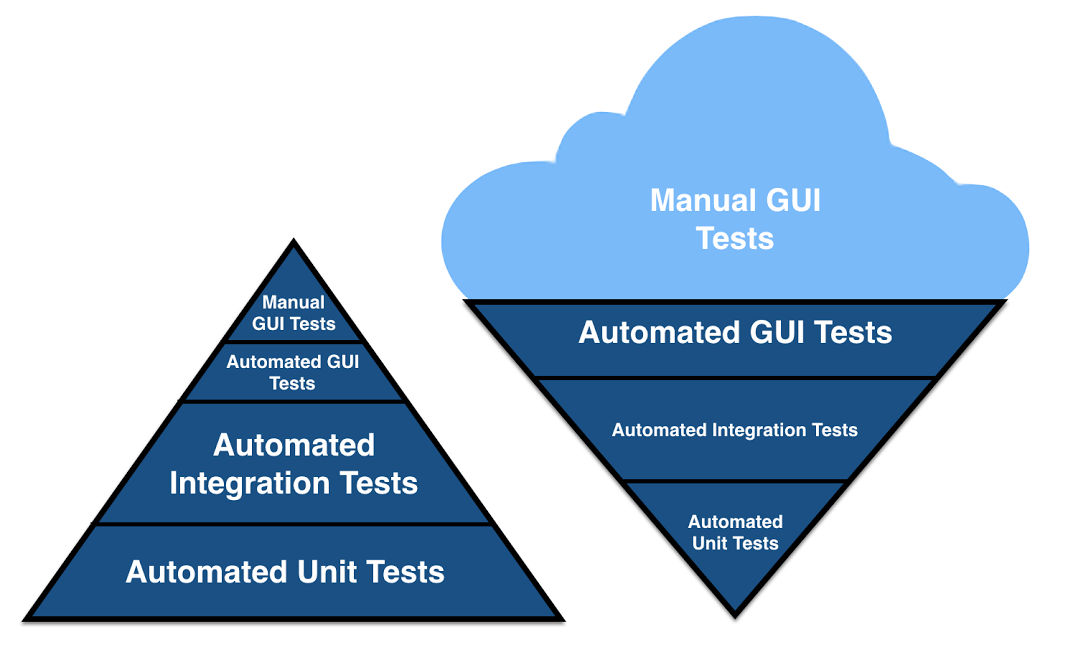
\includegraphics[width=1\textwidth]{img/ext/testing_pyramid.png}
	\caption[Srovnání strategie \enquote{testovací pyramidy} a \enquote{zmrzlinového kornoutu}]{Srovnání strategie \enquote{testovací pyramidy} (vlevo) a \enquote{zmrzlinového kornoutu} (vpravo) \cite{test-fishman}}\label{fig:testing_pyramid}
\end{figure}

Konkrétní aplikace této strategie závisí na vlastnostech projektu, týmu a požadavcích. Přesto se pokusím uvést obecná doporučení různých autorů. Čím níže z pohledu test pyramidy se podaří vývojářům dostat, tím lépe pro budoucí práci -- lépe začít např. s API, než s UI -- případně lze pracovat ve více lidech na více úrovních paralelně \cite{test-kitner}. Pokud ale aplikace už běží a postrádá jakékoliv testy, je ideální začít s tvorbou testů na vrcholu pyramidy pro kritické klíčové části byznysu \cite{test-atlassian}. Pro zbytek je vhodné využít nižší úrovně testů \cite{test-atlassian2}.

Mnoho organizací má i přes testovací pyramidu většinu automatizovaných testů postavených nad UI vrstvou \cite{test-devqa}, výhodou je dohled nad výsledným produktem, který je pak používán, nevýhodou křehkost a nesnadné dohledávání původu chyb zachycených při testech UI, v případě použití AJAX (Asynchronous JavaScript and XML) je také mnohem složitější vytvořit deterministické UI testy \cite{test-timothy}. Testovací pyramida je pak obrácená a obvykle se tomuto přístupu vzhledem k tvaru obrácené pyramidy říká \enquote{zmrzlinový kornout} \cite{test-mf1}, viz opět obrázek~\ref{fig:testing_pyramid}. 

Při volbě správné části k testování je třeba řídit se tím, která část je pro byznys zákazníka důležitá \cite{test-kitner}, než pouze například co nejvyšším pokrytím kódu testy \cite{test-devqa}. V případě, že se UI testy použijí pro klíčové funkce aplikace, můžeme zajistit, že i přes případné drobnější chyby funguje ta nejdůležitější část aplikace korektně, a to včetně všech vrstev jako např. napojení na API, databázi ad., to umožní častější dodávání nových verzí zákazníkovi s větší jistotou fungování, to vše je ale třeba dělat s vědomím jednotlivých úrovní testovací pyramidy a důsledků použití UI testů \cite{test-novanet}. Je tedy vhodné ve vyšší vrstvě testovat dva typy průchodů -- nejhorší a nejideálnější -- a pro zbytek hraničních případů využít vrstvy nižší \cite{test-dzone}.

Strategie testovací pyramidy je často špatně interpretována a může například vyústit v napsání naprosto všech možných unit testů a poté přesunutí do vyšší vrstvy atd., což pro některé týmy může být vhodné, pro jiné ale zbytečně komplexní a drahé \cite{test-cucumber2}. Principem pyramidy je naznačit, že testů na vyšší vrstvě má být méně než na nižší \cite{test-cucumber2}. Ačkoliv se princip testovací pyramidy stává standardem pro agilní týmy, je třeba rozumět principům, se kterými tento přístup přichází a na základě zavést způsoby testování pro konkrétní projekt \cite{test-cucumber2}. Na závěr je třeba říci, že veškeré zmíněné termíny, názvy a definice nejsou rigorózní a často panují různé názory např. na rozdělení testovací pyramidy, definici UI testování (někdy synonymum end-to-end testování, někdo nikoliv z toho důvodu, že UI lze testovat i pomocí unit testů) a mnoho dalšího, při tvorbě testů v rámci softwarového produktu je tedy vždy třeba jasně vymezit a definovat rozsah testů, sjednotit terminologii a na všem se domluvit \cite{test-fowler}.

\subsection{Alternativní přístupy}

Alternativním přístupem pro testování klientské části je strategie tzv. \enquote{testovací trofeje} \cite{test-trophy}, která se skládá ze 4 částí, od té nejnižší: statické testy (založené na statickém typování a linterech, viz TODO), unit testy (cílené na kritické části aplikace), integrační testy (ověřující, že vše spolu korektně spolupracuje) a end-to-end funkční testy (simulace chování uživatele při důležitých průchodech aplikací prostřednictvím automatizovaného klikání -- tedy UI testy z testovací pyramidy). Jak ale opět uvádí \cite{test-roth}, tento přístup opět může pro některé týmy a aplikace být vhodný, pro některé nikoliv a bez dostatečné znalosti konkrétního kódu aplikace a problematiky může následování nejen tohoto vzoru vyústit ve slepou cestu.

\begin{figure}[h]\centering
	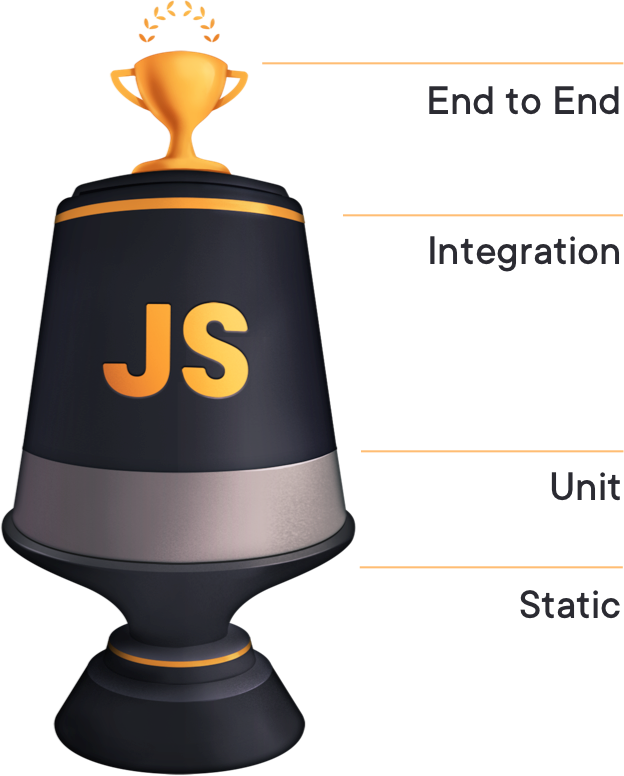
\includegraphics[width=0.4\textwidth]{img/ext/testing_trophy.png}
	\caption[Strategie \enquote{testovací trofeje}]{Strategie \enquote{testovací trofeje} \cite{test-trophy}}\label{fig:testing_trophy}
\end{figure}

\section{Metodiky a nástroje pro automatizované testování}

Svět testování je ovlivňován několika metodikami vývoje softwaru, především TDD (Test-Driven development) a BDD (Behaviour-Driven development) \cite{test-swtestinghelp1}. S těmito metodikami souvisí také různé nástroje pro automatizované testování podporující příslušný způsob vývoje, o nich se též zmíním. Na závěr uvedu ještě další nástroje pro UI testování.

\subsection{TDD}

Základním principem TDD je napsat nejprve testovací případy (přímo v programovacím jazyce) a až poté implementovat kód, který zařídí splnění těchto případů \cite{test-swtestinghelp2}. Výsledkem je vyšší kvalita a flexibilita kódu (tím pádem lze pak jednoduše provádět např. refaktoring) a také vysoké pokrytí kódu \cite{test-swtestinghelp2}. Nevýhodou TDD je, že změny ve fungování aplikace mohou mít velký dopad na testovací případy, testovacím případům také rozumí pouze lidé se znalostí programovacích jazyků \cite{test-swtestinghelp2}. Vzhledem k zaměření testů na konkrétní implementaci a nikoliv chování je ale snadnější najít v případě TDD testů konkrétní chybu  \cite{test-swtestinghelp2}. TDD testy se zaměřují zejména na nejnižší vrstvu v testovací pyramidě, tedy unit testy \cite{test-swtestinghelp1}, principy TDD se ale mohou aplikovat napříč všemi vrstvami \cite{test-dzone}.

Mezi nástroje pro podporu TDD patří xUnit frameworky, např. \href{https://junit.org/}{JUnit}, \href{https://testng.org/}{TestNG}, \href{https://nunit.org/}{NUnit} \cite{test-swtestinghelp2}. Pro JS se dle \cite{test-chart-js2} a \cite{test-chart-js1} nejvíce používá \href{https://jestjs.io/}{Jest} a \href{https://mochajs.org/}{Mocha}, pro Python se používá \href{https://docs.pytest.org/en/latest/}{PyTest} nebo \href{https://docs.python.org/3/library/unittest.html}{unittest} \cite{test-chart-python}.

\subsection{BDD}

BDD rozšiřuje TDD a místo psaní testovacích případů se zapisují požadované scénáře chování, později je opět implementován samotný kód aplikace zařizující její předem specifikované chování \cite{test-swtestinghelp2}. Díky zápisu scénářů v jazyce Gherkin, který vychází z přirozeného jazyka, je možná jednoduchá spolupráce mezi vývojáři, testery, analytiky a zákazníkem (i bez znalosti programovacích jazyků) \cite{test-swtestinghelp2, test-cucumber1}, vytvořené scénáře tvoří prakticky základ pro dokumentaci funkcí aplikace \cite{test-smartbear2}. Při vývoji aplikace totiž často dochází k nedorozuměním ohledně výkladu různých požadavků. Výhodou BDD je také zaměření na samotné chování aplikace, nikoliv na přemýšlení o implementaci v kódu, chování aplikace je hlavní prvek, na který se vývojáři a testeři zaměřují a umožňuje to tak držet se lépe požadavků zákazníka \cite{test-swtestinghelp2}. BDD testy se zaměřují zejména na prostřední vrstvy v testovací pyramidě, tedy API testy \cite{test-swtestinghelp1}.

Mezi nástroje pro podporu BDD patří frameworky jako \href{https://specflow.org/}{SpecFlow}, \href{https://cucumber.io/}{Cucumber}, \href{https://github.com/machine/machine.specifications}{MSpec} \cite{test-swtestinghelp2}. Ze scénářů lze vytvářet vždy aktuální dokumentaci a reporty díky nástrojům jako \href{https://smartbear.com/product/testcomplete/overview/}{TestComplete} \cite{test-smartbear2}. Pro JS se používá \href{https://cucumber.io/docs/installation/javascript/}{Cucumber.js}, pro Python se používá \href{https://behave.readthedocs.io/en/latest/}{Behave} \cite{test-chart-bdd}.

BDD se často používá spolu s TDD, protože dokáže na vyšší úrovni prověřit korektní fungování aplikace a poskytnout tak vyšší důvěru ve výsledný produkt \cite{test-cucumber1} -- takové testy tedy prověří nějaké chování aplikace a doplněním o TDD testy na nižších úrovních se dotestují specifické části.

\subsection{Další nástroje}

Jak jsem již zmínil, BDD se zaměřuje na vyšší vrstvy testovací pyramidy, pro UI testování se tedy často používá s nástroji jako \href{https://www.selenium.dev/}{Selenium} \cite{test-dzone}. Selenium je sada nástrojů a knihoven pro automatizované testování webových aplikací \cite{test-seleniumdocs}. Prostřednictvím tzv. WebDriveru, který je implementován jednotlivými tvůrci prohlížečů, umožňuje interagovat s webovou stránkou v prohlížeči (a to nejen v běžném módu, ale také tzv. \enquote{headless} módu, kde prohlížeč běží bez GUI) \cite{test-hackernoon1, test-seleniumdocs}. Pro \enquote{headless} mód byl do nedávné doby nejpopulárnější volbou \href{https://phantomjs.org/}{PhantomJS}, vzhledem k postupné implementaci této funkce do předních webových prohlížečů byl ale jeho vývoj zastaven a přechází ze na běžné prohlížeče, protože právě v těch koncový uživatel pracuje \cite{test-fowler, test-phantomjs}.

Selenium je mocný nástroj, nevýhodou je ale poměrně zdlouhavý zápis skriptů pro výběr elementů, práci s výjimkami a časováním, proto se často volí nádstavby zaobalující Selenium, které umožňují jednodušší zápis a práci, např. \href{https://selenide.org/}{Selenide} \cite{test-hackernoon1}. Také je možné využít komplexní testovací frameworky, které nabízí mnohem více nástrojů pro práci s testy, z nichž některé jsou také postavené na Seleniu, z mnohých používaných například \href{https://www.katalon.com/}{Katalon Studio} či \href{https://robotframework.org/}{Robot framework} \cite{test-selenium3, test-katalon}.

Selenium se postupem času stalo průmyslovým standardem pro UI testování, a to zejména díky jednoduchosti použití, kompatibilitě (s mnoha prohlížeči, možnost použití s mnoha programovacími jazyky) a popularitě \cite{test-selenium1}. Jak ale uvádí \cite{test-cypress1}, v případě asynchronních aplikací je Selenium složitější používat vzhledem k principu jeho fungování, protože je třeba vždy explicitně čekat na objevení elementu na stránce, problémem ale je, že nevíme, jak dlouho čekat. I z toho důvodu zde autor nabízí alternativu v podobě novějšího \href{https://www.cypress.io/}{Cypress}, který nabízí mnohem lepší práci s asynchronními aplikacemi, problémem ale je možnost použití pouze s JS, malá komunita a popularita, méně návodů \cite{test-cypress1}. Další nevýhodou Cypress byla podpora výhradně prohlížeče Google Chrome, to se ale v únoru 2020 změnilo \cite{test-cypress2}, naopak výhodou uváděnou např. v \cite{test-cypress3} byla lepší dokumentace oproti Seleniu, dokumentace Selenia ale byla kompletně přepsána a na podzim 2019 nasazena \cite{test-selenium2}.

\chapter{Konfigurace více prostředí}

tudle kapitolu možná nezařadím a rovnou popíšu způsob řešení v praktické části
obsah: Deployment environments a s tím související Release management

\begin{itemize}
\item přehled toho, jak se můžou řešit různý prostředí, např. staging, testing, produkce apod., asi se tomu rika deployment pipeline
\end{itemize}
\begin{itemize}
\item přehled toho jak s tím souvisí releasy, co kam může jít a k čemu je to dobrý, jak se to dá různě dělat a souvislosti (např. nemusí to dělat travis na základě releasu, ale třeba na základě podmínky proměnné prostředí nebo branch production apod.)f
\end{itemize}

viz:

\begin{itemize}
\item https://continuousdelivery.com/implementing/patterns/\#the-deployment-pipeline
\item https://en.wikipedia.org/wiki/Deployment\_environment
\item https://docs.gitlab.com/ee/ci/environments.html
\item https://cs.wikipedia.org/wiki/Release\_management
\item https://docs.microsoft.com/cs-cz/aspnet/web-forms/overview/deployment/configuring-server-environments-for-web-deployment/scenario-configuring-a-staging-environment-for-web-deployment
\item http://guides.beanstalkapp.com/deployments/best-practices.html
\item ...
\end{itemize}

\chapter{Nástroje pro usnadnění vývoje a údržby}

Postupem času v rámci dalšího vývoje a rozšiřování aplikace se ukázalo, že je třeba použít pokročilé nástroje pro usnadnění samotného vývoje a údržby. Cílem této sekce je nastínit způsob jejich výběru. Jedním z hlavních požadavků je, aby vše potřebné bylo zdarma, neuvažuji zde tedy nástroje nenabízející alespoň nějakou formu bezplatného používání na dobu neurčitou (tedy nikoliv jen pro studenty). Při procházení ceníků budu brát také v úvahu fakt, že repozitář s projektem je open-source (to je jeden z cílů této práce). Při volbě nástrojů pro daný účel budou případně specifikovány další požadavky. Na základě průzkumu pak uvedu nalezené nástroje, jejich vlastnosti a seřadím je orientačně podle popularity na základě stránky \href{https://stackshare.io/}{StackShare}, která poskytuje \cite{stackshare} možnost sdílet používané nástroje a technologie firem a jednotlivců pro jejich projekty, nástroje a technologie srovnávat, hodnotit, řadit dle popularity apod.

\section{Monitorování chyb}
Pro každou aplikaci je důležité monitorovat chyby, díky tomu (nehledě na to, zda uživatel nahlásí problém a bude jakkoliv konkrétní) je možné pak chyby snadněji reprodukovat a opravit \cite{tools-exception}. Nástroje pro monitorování chyb umožňují upozornit vývojáře na výskyt chyby, poskytnout mu kompletní informace o chybě a kontextu, ve kterém nastala \cite{tools-exception}.

Minimální požadavky jsou:
\begin{itemize}
    \item zdarma pro použití na neomezenou dobu jak na Heroku (aplikace v rámci této práce), tak mimo Heroku (další aplikace např. v rámci ÚP) -- tento požadavek je zde kvůli existenci nástrojů jako např. \href{https://airbrake.io/}{Airbrake}, který na Heroku nabízí plán zdarma \cite{airbrake-heroku}, ale ve svém ceníku jej nenabízí \cite{airbrake-pricing}, tedy tyto nástroje neuvažuji,
    \item SaaS (Software as a Service) -- tedy aplikace hostovaná provozovatelem služby \cite{oracle-saas},
    \item možnost použití pro klientskou (JS s Reactem) i serverovou část (Python s Djangem).
\end{itemize}

Pro monitorování chyb existuje mnoho nástrojů, podle StackShare \cite{stackshare-exception} volím 4 nejpoužívanější, které splňují všechny požadavky. I přes mnoho dalších funkcionalit těchto nástrojů se zde zaměřuji na primární účel, tedy monitorování chyb -- nehledě na to, jaké další integrace a funkce jsou poskytnuty zdarma.

Nejpoužívanější nástroje podle StackShare (řazeno od nejpoužívanějšího) \cite{stackshare-exception} splňující zmíněné požadavky:
\begin{enumerate}
    \item \href{https://sentry.io/}{\textbf{Sentry}}: zdarma nabízí 5~000 událostí/měsíc pro neomezený počet projektů, 7~dní historie dat \cite{sentry-pricing}, podporuje React i Django \cite{sentry-platforms},
    \item \href{https://rollbar.com/}{\textbf{Rollbar}}: zdarma nabízí 5~000 událostí/měsíc pro neomezený počet projektů, 30~dní historie dat \cite{rollbar-pricing}, podporuje React i Django \cite{rollbar-platforms},
    \item \href{https://www.bugsnag.com/}{\textbf{Bugsnag}}: zdarma nabízí 7~500 událostí/měsíc pro neomezený počet projektů, 7~dní historie dat \cite{bugsnag-pricing}, podporuje React i Django \cite{bugsnag-platforms},
    \item \href{https://www.honeybadger.io/}{\textbf{Honeybadger}}: zdarma nabízí 12~000 událostí/měsíc pro neomezený počet projektů, 15~dní historie dat \cite{honeybadger-pricing}, podporuje React \cite{honeybadger-react} i Django \cite{honeybadger-django}.
\end{enumerate}

Jiný přístup k monitorování chyb na klientské části nabízí nástroje jako \href{https://logrocket.com/}{LogRocket} -- ten k zachyceným chybám přidá i nahrané video s kroky uživatele vedoucími k dané chybě (ve videu je obrazovka zachycující přesně to, co uživatel viděl) \cite{logrocket}. LogRocket nabízí zdarma 1~000 nahraných sezení uživatelů/měsíc (sezení je jedno kontinuální používání aplikace daným uživatelem) \cite{logrocket-pricing}, 14~dní historie dat, podporuje React \cite{logrocket-react}.

\section{Správa logů}
% todo pravidlo https://12factor.net/logs
Nasazené aplikace generují mnoho logů z různých procesů, v případě Heroku jsou všechny tyto logy agregovány do jednoho kanálu a nabízí možnost uchování posledních 1~500 logů nejdéle 1~týden \cite{tools-logs1}. V případě, že chceme přístup k většímu počtu logů či ke starším, je třeba využít buď možnost napojení logů na některý z doplňků na Heroku, případně logy rovnou přímo přesměrovávat do jiné služby \cite{tools-logs1}. Tyto nástroje pro správu logů pak umožňují spravovat velké množství agregovaných logů generovaných z mnoha typů zařízení a serverů -- nad nimi provádět mj. různé dotazy, vyhledávání, pohledy, případně i analýzy či upozornění na nějaké události \cite{tools-logs2}.

Minimální požadavky jsou:
\begin{itemize}
    \item zdarma pro použití na neomezenou dobu pro logy z Heroku,
    \item SaaS -- tedy aplikace hostovaná provozovatelem služby \cite{oracle-saas},
    \item upozorňování na události e-mailem,
    \item historie logů alespoň na 7 dnů.
\end{itemize}

Pro správu logů existuje mnoho nástrojů, podle StackShare \cite{stackshare-log} volím 2 nejpoužívanější, které splňují všechny požadavky. I přes mnoho dalších funkcionalit těchto nástrojů se zde zaměřuji na primární účel, tedy ukládání logů, vyhledávání a upozorňování -- nehledě na to, jaké další funkce jsou poskytnuty zdarma (během hledání se ukázalo, že právě požadavek upozorňování většina nástrojů zdarma neposkytuje, filtrem dle požadavků tedy nakonec prošly pouze 2 nástroje).

Nejpoužívanější nástroje podle StackShare (řazeno od nejpoužívanějšího) \cite{stackshare-log} splňující zmíněné požadavky:
\begin{enumerate}
    \item \href{https://www.papertrail.com/}{\textbf{Papertrail}}: zdarma nabízí 50~MB logů/měsíc, 7~dní historie logů (vyhledávání ale jen pro poslední 2~dny), nastavitelná upozornění \cite{papertrail-pricing}, možnost použít Heroku doplněk pro jednoduché nastavení (nabízí dokonce více uložených logů -- 10~MB logů/den) \cite{heroku-papertrail},
    \item \href{https://logentries.com/}{\textbf{Logentries}}: zdarma nabízí 5~GB logů/měsíc, 7~dní historie logů \cite{logentries-pricing}, nastavitelná upozornění \cite{logentries-pricing2}, možnost použít Heroku doplněk pro jednoduché nastavení \cite{heroku-logentries}.
\end{enumerate}


\section{Statické typování}
moznosti, ze python ma builtin, JS nema (uvest proc, viz ecma vyjadreni), jak se to v JS resi a srovnat: FlowJS, Typescript + jak jsou na tom ostatni jako coffeescript, dart, kotlin..; u TS zminit podporu babel

\subsection{Klientská část}


\subsection{Serverová část}

\section{Statická analýza kódu}
Statická analýza kódu je efektivní nástroj pro posouzení kvality kódu (např. konzistence, čitelnost, zranitelnosti, výkon, pokrytí testy) projektu a předvídání potenciálně vznikajících problémů (tzv. \enquote{code smells}) bez spuštění samotného kódu \cite{medium-devgurus, static-overops}. Samotný kód je analyzován vůči sadě pravidel a standardů \cite{static-overops}

Na základě průzkumu nástrojů zde zavádím vlastní dělení na nástroje představující vyšší a nižší vrstvu analýzy kódu, vysvětlení důvodů vedoucích k tomuto dělení následuje vzápětí.

V první podsekci se zaměřím na rešerši nástrojů na vyšší vrstvě, které umožňují průběžnou kontrolu kvality kódu. Jak je vidět z \cite{guru-codereview, gh-awesomecodereview, medium-devgurus,stackshare-codereview, gh-awesomecodereview2}, v této oblasti není úplně jednoznačná terminologie -- těmto nástrojům se často též říká nástroje pro posuzování kvality kódu, zaměřují se třeba i na pokročilou práci s manuálním posuzováním kódu ad., někdy se též nazývají nástroje pro \textit{automatické} posuzování kvality kódu, což už je k této sekci bližší. V této první podsekci se tedy zaměřím na ty nástroje, které poskytují právě automatickou průběžnou kontrolu kvality kódu a dávají poté zpětnou vazbu pro kód aplikace.

Ve druhé podsekci se zaměřím na nástroje z nižší vrstvy (tzv. lintery), na kterých často nástroje z vyšší vrstvy stavějí (proto také dělení na vyšší a nižší vrstvu pro lepší orientaci). Tyto nástroje se používají při samotném vývoji na lokálním zařízení a poté se mohou spouštět např. na integračním serveru.

\subsection{Průběžná kontrola kvality kódu}

Na zmíněné vyšší vrstvě se nalézají nástroje, které jsou provozované jako služby automaticky kontrolující kvalitu kódu. Obvykle jsou to služby typu SaaS, případně On-Premise (tedy opak SaaS \cite{globema-onpremise}) \cite{codebeat-engines}. Tyto nástroje lze do procesu vývoje zapojit a zlepšovat tak kvalitu kódu už od počátku -- např. nastavit hranice pro kvalitu kódu vzhledem k pokrytí kódu testy a nulovému počtu nalezených problémů, na základě toho se pak může třeba PR (Pull Request) změn automaticky označit jako úspěšný nebo nikoliv \cite{medium-devgurus}. To pak snižuje množství diskuzí mezi vývojáři, protože je zavedeno objektivní hodnocení kódu \cite{medium-devgurus}. Nejprve uvedu minimální požadavky na nástroje pro zúžení výběru:
\begin{itemize}
    \item zdarma pro použití na neomezenou dobu,
    \item integrace s GitHub,
    \item podpora JS, TS (TypeScript) a Python (ne nutně všech naráz),
    \item SaaS -- tedy aplikace hostovaná provozovatelem služby \cite{oracle-saas}.
\end{itemize}

Při průzkumu těchto nástrojů jsem zjistil, že se prakticky dají dále rozdělit do dvou typů:
\begin{enumerate}
    \item Nástroje založené z valné většiny především na integraci mnoha různých nástrojů z nižší vrstvy (lintery), případně pouze na základních pravidlech pro kontrolu kódu jako např. délka metod, počet řádků souboru, složitost metod, duplikace apod. Jak uvádí \cite{globema-onpremise}, některé nástroje upřednostňují vytvoření vlastních pravidel místo integrace nástrojů kvůli lepší rozšířitelnosti a správě pravidel, ve výsledku pak tedy nabízejí alternativu ke službám integrující všechny standardní nástroje. Možná je také kombinace obou přístupů nebo funkce pro vytváření vlastních jednoduchých pravidel na míru projektu.
    \item Nástroje založené na pokročilé hloubkové analýze kódu různými způsoby. Ty mohou být doplněné o možnost vytváření vlastních stejně pokročilých pravidel na míru projektu. Také mohou nabízet volitelnou integraci nástrojů z nižší vrstvy.
\end{enumerate}

Zde je na místě okomentovat, proč je toto rozdělení důležité. Nástroje prvního typu prakticky jen sdružují mnoho různých nástrojů na jednom místě, jejichž výsledky agregují a třídí přehledně na jednom místě. Právě toto sjednocení různých nástrojů do jedné služby je jejich přidaná hodnota oproti tomu, kdy by vývojář tyto nástroje spouštěl jednotlivě. Nástroje druhého typu nabízejí pokročilou hloubkovou kontrolu kódu způsobem, jakým to běžné lintery, na kterých stojí nástroje prvního typu, nezvládnou \cite{deepscan-lintercompare}. Díky tomu umožňují vyhledat velmi závažné problémy, chyby či zranitelnosti, které by jinak mohly být opomenuty \cite{deepscan-lintercompare, deepsource2}. To zvládnou díky vlastním pokročilým pravidlům a analýzám založených např. na umělé inteligenci \cite{deepsource2} apod. Jejich výhodou také je, že obvykle najdou reálné problémy místo mnoha nedůležitých, které mohou poskytnout nástroje prvního typu -- tuto myšlenku vystihují autoři DeepSource \cite{deepsource2}: \enquote{\textit{DeepSource is designed to understand the context of your code and filter out the noise from the results. This prevents warning blindness and encourages developers to take action on issues that matter.}}

Nástroje prvního typu splňující minimální požadavky:
\begin{itemize}
    \item \href{https://www.codacy.com}{\textbf{Codacy}}: zdarma \cite{codacy-pricing}, podporuje JS, TS i Python \cite{codacy-langs}, GitHub integrace pro PR i commity \cite{codacy-gh}, založeno na integraci mnoha nástrojů do jedné služby \cite{codacy-engines},
    \item \href{https://codeclimate.com}{\textbf{Code Climate}}: zdarma \cite{codeclimate-pricing}, podporuje JS, TS i Python \cite{codeclimate}, GitHub integrace pro PR i commity \cite{codeclimate-gh}, založeno na integraci mnoha nástrojů do jedné služby a dalších základních pravidel \cite{codeclimate-engines},
    \item \href{https://www.codefactor.io}{\textbf{CodeFactor}}: zdarma \cite{codefactor-pricing}, podporuje JS, TS i Python \cite{codefactor}, GitHub integrace pro PR i commity \cite{codefactor}, založeno na integraci mnoha nástrojů do jedné služby a dalších základních pravidel \cite{codefactor-engines},
    \item \href{https://www.code-inspector.com}{\textbf{Code Inspector}}: zdarma \cite{codeinspector-pricing}, podporuje JS, TS i Python \cite{codeinspector}, GitHub integrace pro PR i commity \cite{codeinspector}, založeno pouze na základních pravidlech \cite{codeinspector, codeinspector-engines},
    \item \href{https://codebeat.co}{\textbf{codebeat}}: zdarma \cite{codebeat-pricing}, podporuje JS, TS i Python \cite{codebeat}, GitHub integrace pro PR i commity \cite{codebeat}, založeno pouze na základních pravidlech \cite{codebeat-engines},
    \item \href{https://houndci.com}{\textbf{HoundCI}}: zdarma \cite{houndci}, podporuje JS, TS i Python \cite{houndci}, GitHub integrace jen pro PR \cite{houndci}, založeno na integraci mnoha nástrojů do jedné služby \cite{houndci-engines},
    \item \href{https://sider.review}{\textbf{Sider}}: zdarma \cite{sider-pricing}, podporuje JS, TS i Python \cite{sider-engines}, GitHub integrace jen pro PR \cite{sider}, založeno na integraci mnoha nástrojů do jedné služby a vytváření vlastních pravidel na míru projektu \cite{sider-engines}.
\end{itemize}

Nástroje druhého typu splňující minimální požadavky:
\begin{itemize}
    \item \href{https://deepsource.io/}{\textbf{DeepSource}}: zdarma \cite{deepsource}, podporuje jen Python \cite{deepsource}, GitHub integrace pro PR i commity \cite{deepsource-docs}, založeno na pokročilé hloubkové analýze kódu \cite{deepsource2},
    \item \href{https://deepscan.io}{\textbf{DeepScan}}: zdarma \cite{deepscan-pricing}, podporuje jen JS a TS (podporuje i React) \cite{deepscan}, GitHub integrace pro PR i commity \cite{deepscan}, založeno na pokročilé hloubkové analýze kódu \cite{deepscan}, možnost integrace ESLint \cite{deepscan-eslint},
    \item \href{https://lgtm.com}{\textbf{LGTM}}: zdarma \cite{lgtm}, podporuje JS, TS i Python \cite{lgtm-faq}, GitHub integrace pro PR i commity (PR analyzuje vždy okamžitě, commity analyzuje jednou denně) \cite{lgtm-faq}, založeno na pokročilé hloubkové analýze kódu, možnost vytváření pokročilých pravidel na míru projektu \cite{lgtm},
    \item \href{https://sonarcloud.io/}{\textbf{SonarCloud}}: zdarma \cite{sonarcloud}, podporuje JS, TS (podporuje i React \cite{sonarcloud-js}) i Python \cite{sonarcloud}, GitHub integrace pro PR i commity \cite{sonarcloud-gh}, založeno na pokročilé hloubkové analýze kódu \cite{sonarcloud2}, možnost připojit i vygenerované reporty z externích nástrojů (linterů) \cite{sonarcloud-engines},
    \item \href{https://www.deepcode.ai/}{\textbf{DeepCode}}: zdarma \cite{deepcode}, nezávislé na jazyku \cite{deepsource2}, GitHub integrace pro PR i commity \cite{deepcode}, založeno na pokročilé hloubkové analýze kódu (používá rozsáhlé strojové učení) \cite{deepcode2}.
\end{itemize}

\subsection{Lintery}

V předchozí sekci jsem uváděl, že některé nástroje (z vyšší vrstvy) z valné většiny staví na integraci mnoha drobnějších nástrojů (z nižší vrstvy), tzv. linterů. Smyslem této sekce je vysvětlit jejich vlastnosti a fungování a poté prozkoumat možnosti linterů pro aplikaci ÚP. 

lintery (ESlint.. + styly airbnb, standardjs, info o spouste pluginech, standardech, vyvoji ve spolupraci s TS)


\section{Formátování kódu}
code formattery (prettier, black...) + souvislost s flake8 apod.


další možné rešerše nástrojů pro:
\begin{itemize}
\item analyza pruchodu aplikaci (google analytics)
\item pripadne nejake pokrocile veci z travisu co se pouzivaji
\item + hledani dead code - python vulture
\item nastroje pro vyvoj frontendu - bakalarka byla postavena na CRA (create-react-app), ktera byla ejectnuta (takze update reactu byl prakticky nemozny), z toho duvodu se nejprv preslo na nastroj nwb, ktery ale pozdeji nebyl udrzovany a doslo ke zkusebni migraci na neutrinojs (souvisi s mozillou) a na vlastni reseni pres webpack - tady bych teda prosel, co tyhle nastroje umoznuji, ze vlastne stavi nad webpackem, ze je to vlastne abstraktni vrstva nad nim, ktera vsechno zjednodusuje, ale nevyhoda je, kdyz ten nastroj neco neumoznuje (viz nwb), tak mas smulu.. takze pak nejdou lintery, nejde TS... zminit moznosti nastroju, jake nastroje jsou, vyhody a nevyhody; v ramci implementace pak zminim cely pribeh s nwb, neutrinojs a custom webpackem, na zaver uvedu proc jsem vse zmigroval na custom webpack ikdyz neutrinojs fungovalo taky
\end{itemize}

\chapter{Zvolené technologie}

Na základě rešerše zvolím technologie, které pak zakomponuji v implementaci do appky - oargumentuji volbu..

tzn:

\begin{itemize}
\item 1. cim testovat a jak
\item 2. jaka prostredi a jak delat releasy, jak to vse bude fungovat (a fakt funguje)
\item 3. zvolene nastroje pro usnadneni vyvoje a udrzby
\end{itemize}